\section{App - iOS}
Um möglichst viele Endnutzer für unser Produkt zu interessieren, war es uns wichtig für die zwei verbreitetsten Smartphone Betriebssysteme Apps zu entwickeln. Da es sich hierfür um neues Terrain handelt, musste mehr Zeit zur Einarbeitung eingeplant werden, als anfänglich gedacht.

\subsection{XCode}
%Stichpunkte:
%IDE: XCode und swift--> hier haben wir die größte Chance zwecks Kompatibilität  :) 
%Phone Simulatoren gibts auch
%gratis IDE

%https://developer.apple.com/de/support/xcode/

\subsection{SwiftUI}
\subsection{Hauptkriterien an die Funktionalität}

Damit die App erkennt, ob sich das Auto bewegt oder nicht, muss sie mit dem Webserver kommunizieren, um sich dort die GPS Daten zu holen. Dazu soll eine Logik eingebaut werden, dass die App eine Abweichung erkennt (wenn Alarmsystem "scharf") und eine Benachrichtigung an den Nutzer sendet. Hier stehen die GPS Daten, die vom Arduino  an den Webserver geschickt werden: http:\/\/retrorbit.spdns.de\/provide\_Data.php

optional: schön wäre es, wenn die GPS Daten nicht als plain Text angezeigt würden sondern direkt in einer Karte, wie man es von Google Maps gewohnt ist.

optional: cool wäre es, wenn die App erkennt, ob der server gerade da ist - dann symbol grün, sonst rot 
--> erst einmal einen Ladekreis eingefügt-damit der user merkt, dass etwas passiert - sieht zumindest erstmal schöner aus und man sieht, dass wir dran gedacht haben :)


\begin{figure} [H]
	\begin{center}
		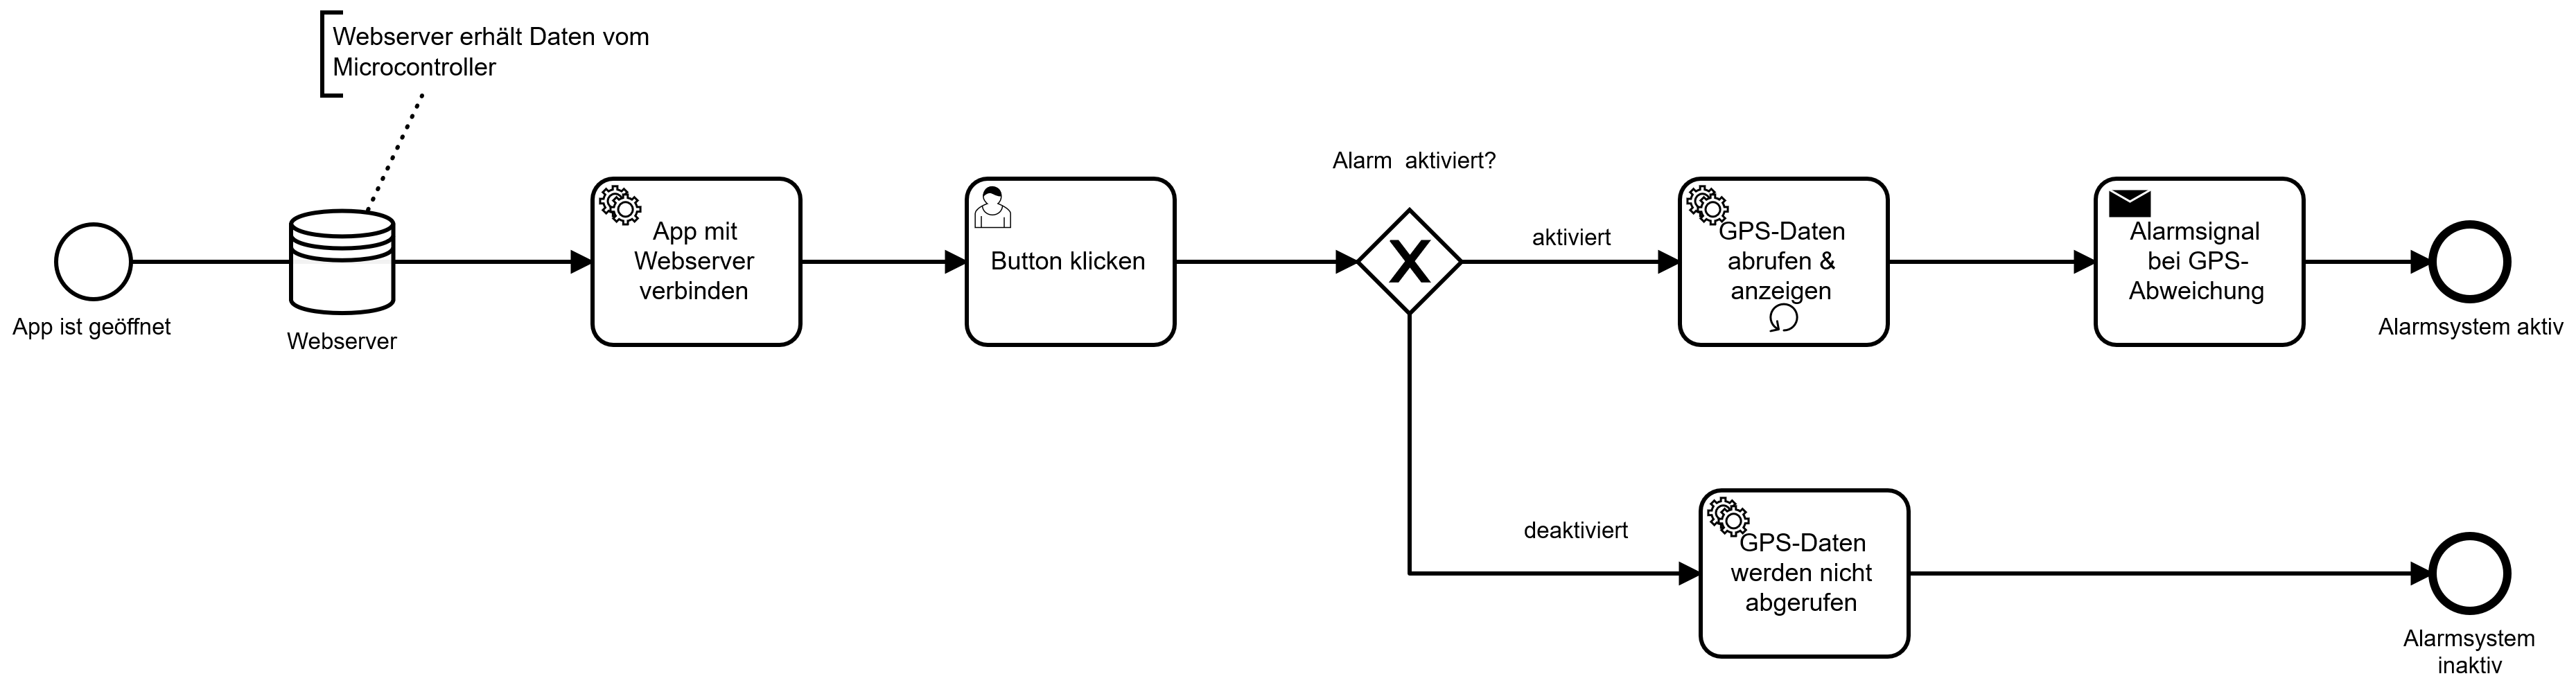
\includegraphics[width=1\textwidth]{Bilder/iOS_camunda.png}
		\caption{Entwurf der iOS-App}
		\label{camunda}
	\end{center}
\end{figure}
\subsection{Design}
%Stichpunkte:
%für imgs: pixabay/com/de --> gratis Bilder, die für apps gentutz werden dürfen


Unscheinbar aber wichtig! Der Nutzer sieht als erstes das AppIcon im Appstore sowie später auf seinem Bildschirm. Hierbei war es uns wichtig, dass dieses Icon nicht nur zu unserem Produkt passt, sondern auch optisch sehr anspricht.
\begin{figure} [H]
	\begin{center}
		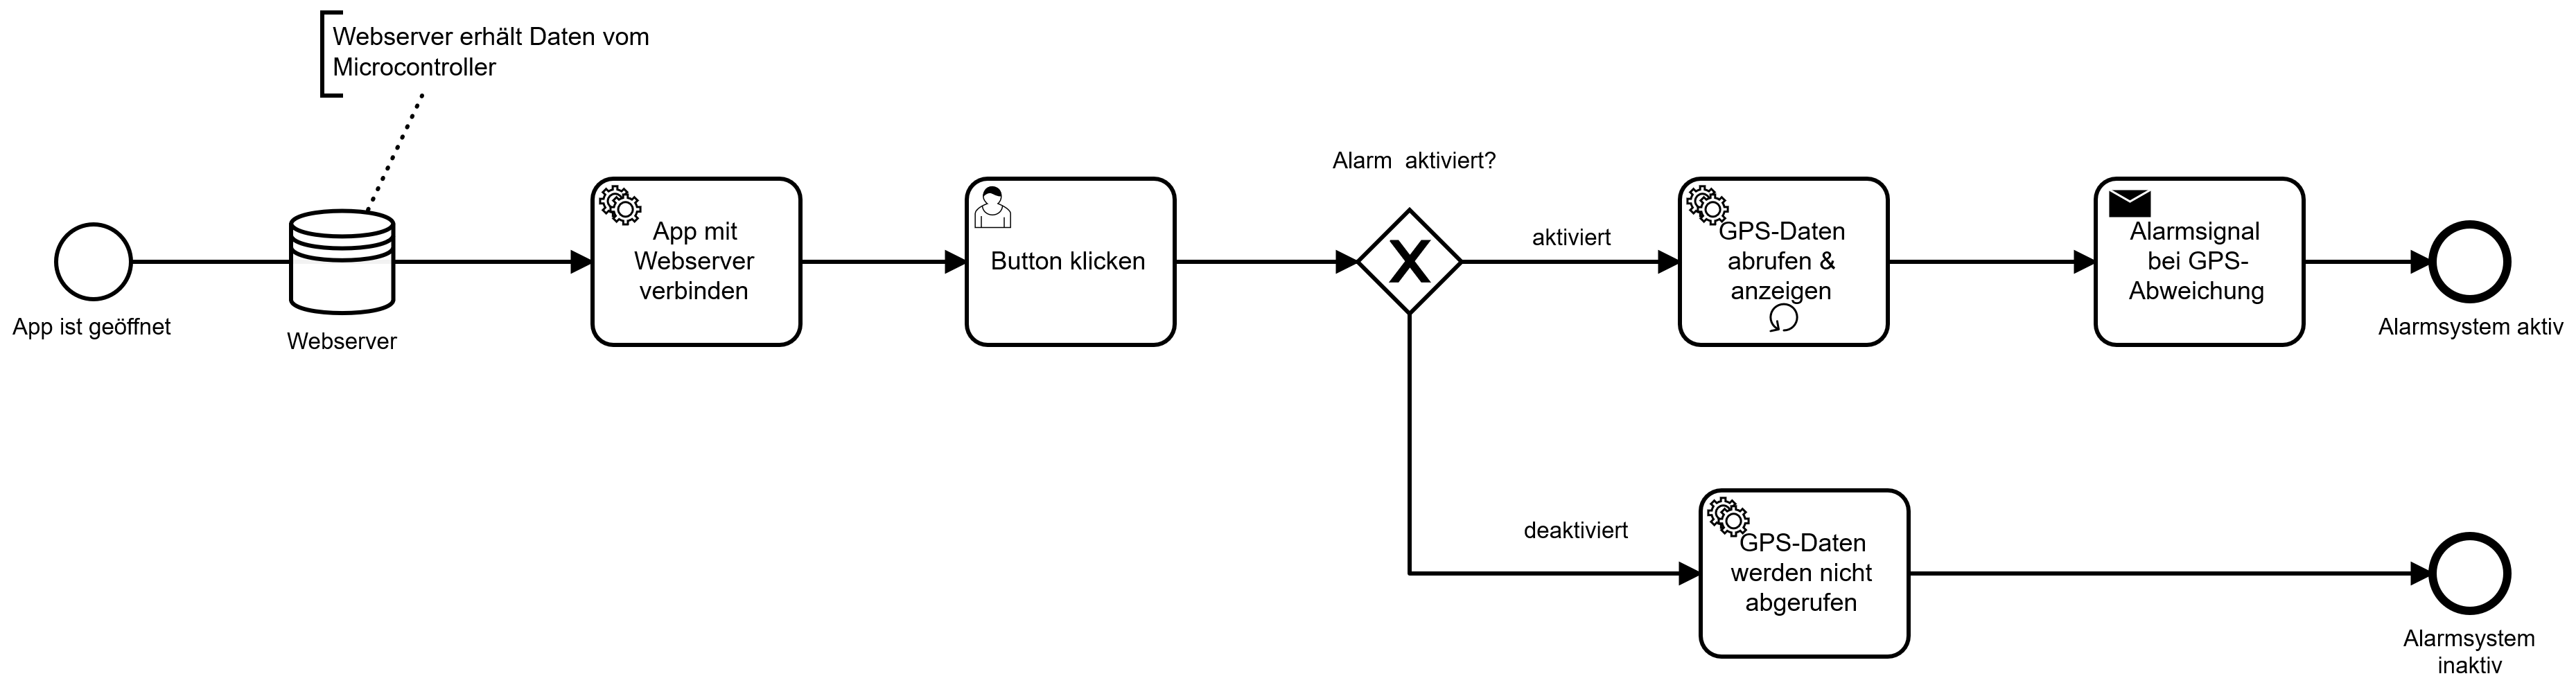
\includegraphics[width=1\textwidth]{Bilder/iOS_camunda.png}
		\caption{AppIcon auf dem Bildschirm}
		\label{AppIcon}
	\end{center}
\end{figure}
Nach dem berühmten Tap auf das Icon hängt es oftmals vom Alter des genutzten Gerätes ab, wie schnell eine App sich aufbaut. Damit auch hier der User ein Feedback erhält, ob  etwas passiert, haben wir einen Launchscreen implementiert, welcher ebenfalls zum restlichen Design der App angepasst wurde.
\begin{figure} [H]
	\begin{center}
		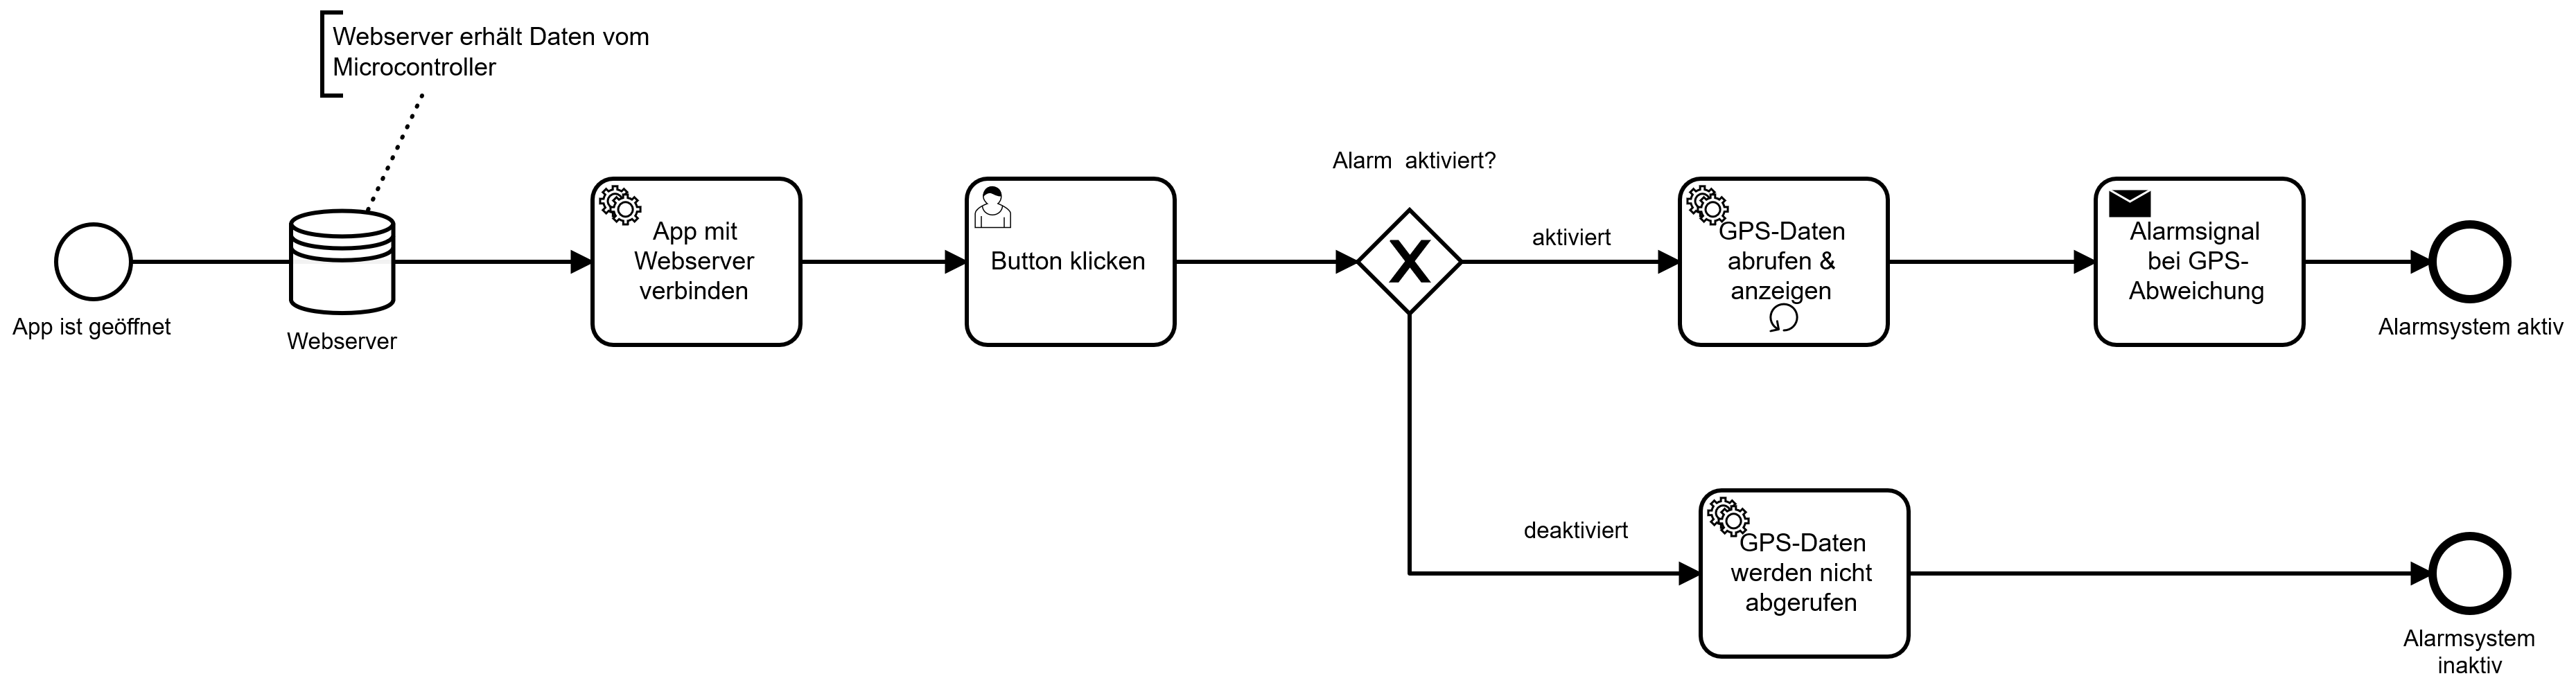
\includegraphics[width=1\textwidth]{Bilder/iOS_camunda.png}
		\caption{Launchscreen}
		\label{Launch}
	\end{center}
\end{figure}

Bei der Umsetzung des Kartendesigns war es wichtig, dass der Nutzer die vom Server bereitgestellten Daten nicht als plain-Text darstellt, sondern die Koordinaten direkt als Standort auf einer Karte übersetzt.
\begin{figure} [H]
	\begin{center}
		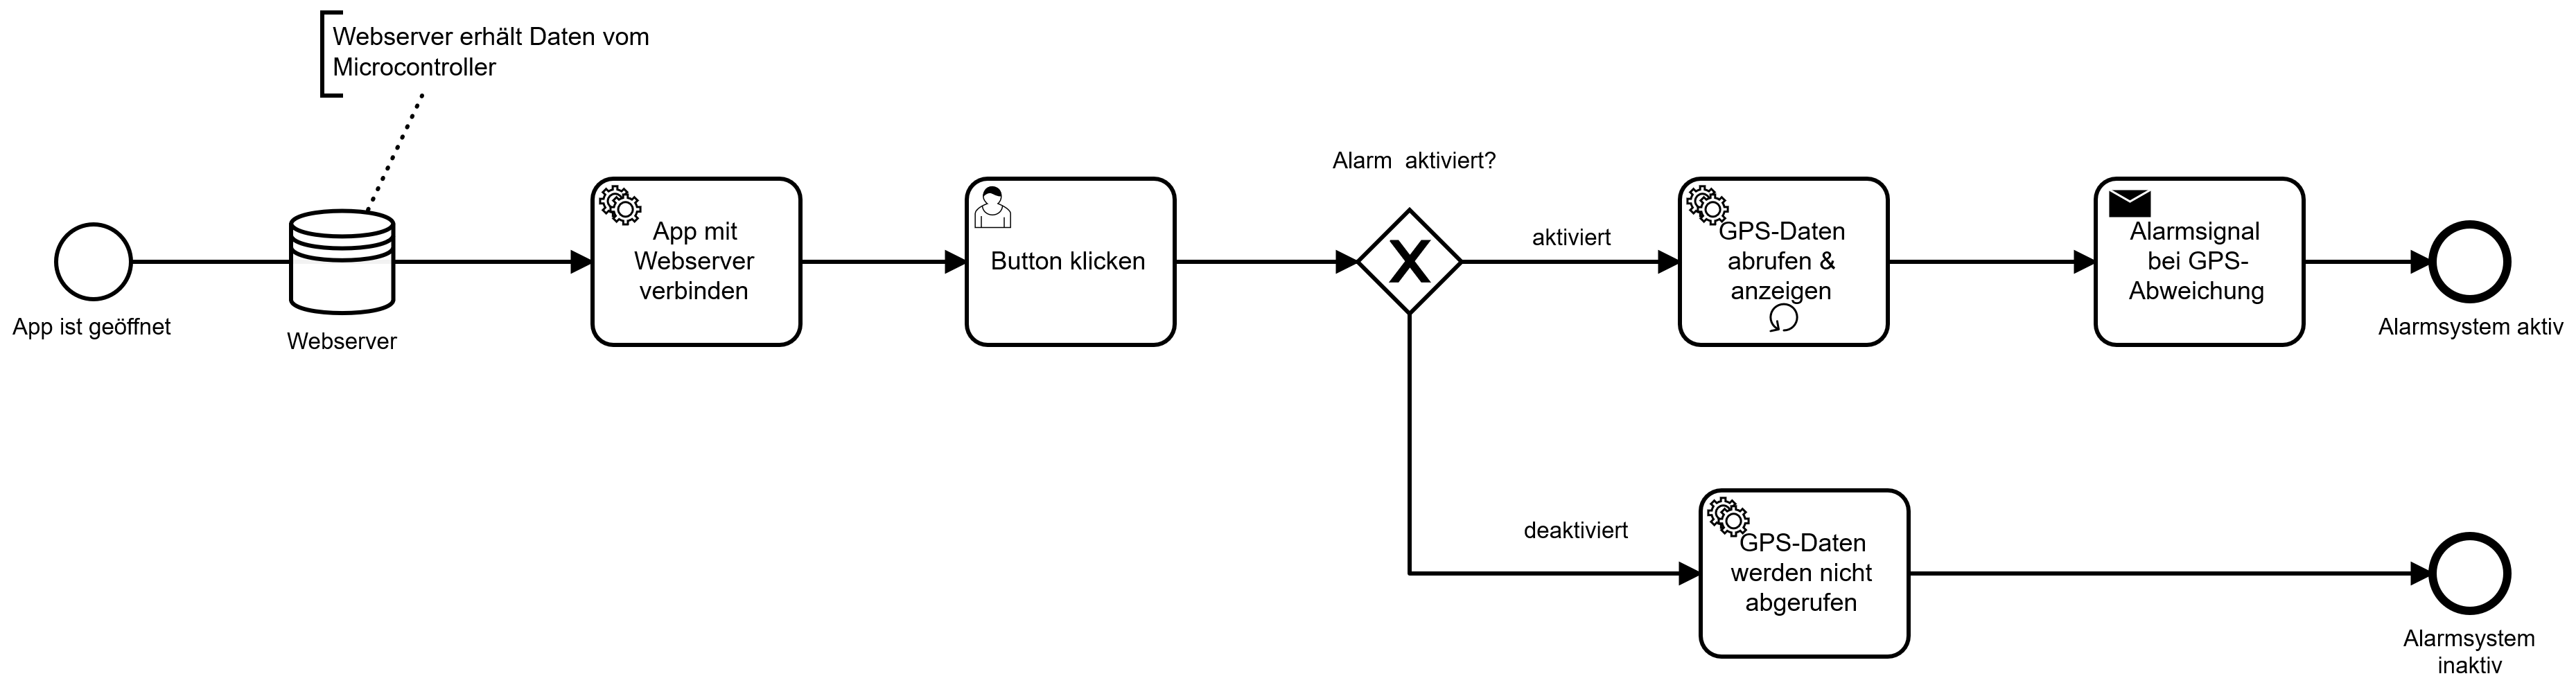
\includegraphics[width=1\textwidth]{Bilder/iOS_camunda.png}
		\caption{Navigationstab \textit{Map}}
		\label{Map}
	\end{center}
\end{figure}



Eine Demonstration der iOS-App kann sich auf der Platform YouTube angesehen werden unter : https://www.youtube.com/watch?v=gWaSZPfxT9s

\subsection{Probleme}
\textbf{Koordinaten in JSON als String hinterlegt:}
\\
Zu Beginn wurden die Koordinaten, sowie der Abrufzeitpunkt als Strings vom Server zur Verfügung gestellt, was ein parsen sehr erschwerte, da für die Verarbeitung dieser Daten die iOS-Map integer beziehungsweise double-Werte benötigt. Dies Problem konnte jedoch nach interner Rücksprache schnell behoben werden, da es sich lediglich um eine Einstellung beim encode des Webservers handelte.

\textbf{Http? Abrufen verboten!}
\\
Die benötigten Daten vom Server werden nicht innerhalb der App angezeigt und es erweckte auch nie den Anschein, dass diese überhaupt abgerufen werden. Es wurde sehr lange das Problem innerhalb der Methoden gesucht, jedoch ohne nennenswerte Erkenntnisse. Erst als extern um Hilfe gebeten wurde, kam schnell heraus, dass SwiftUI den Abruf von JSON-Daten einer Http-Seite verhindert. Bei Nutzung einer anderen JSON-Datei von einer Https-Seite und gezielte Platzierung von print()-Ausgaben im Log ergaben dann das eigentliche Problem
 
\begin{figure} [H]
	\begin{center}
		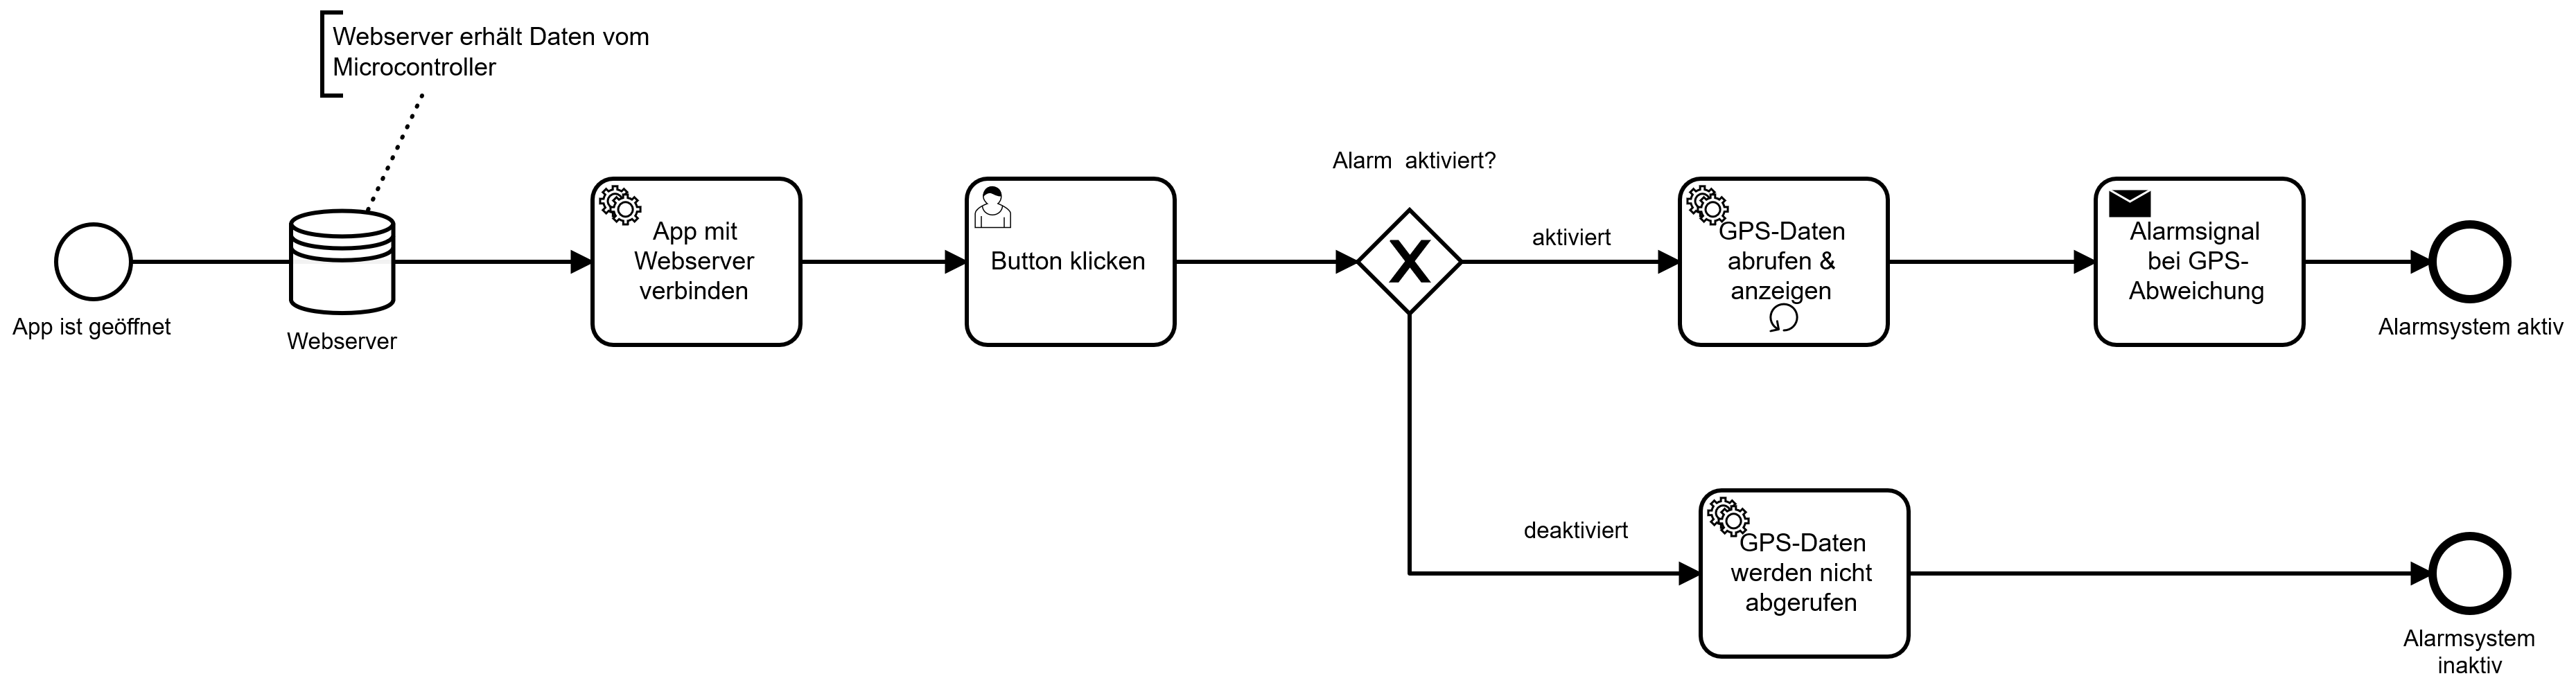
\includegraphics[width=1\textwidth]{Bilder/iOS_camunda.png}
		\caption{Fehlermeldung \textit{NSAppTransportSecurity}}
		\label{fehler}
	\end{center}
\end{figure}
Auf Apple-Plattformen verbessert eine Netzwerkfunktion namens App Transport Security (ATS) den Datenschutz und die Datenintegrität für alle Apps und App-Erweiterungen. ATS erfordert, dass alle HTTP-Verbindungen, die mit dem URL-Ladesystem hergestellt werden – normalerweise unter Verwendung der URLSession-Klasse – HTTPS verwenden. Es erlegt außerdem erweiterte Sicherheitsprüfungen auf, die die vom TLS-Protokoll (Transport Layer Security) vorgeschriebene Standard-Server-Vertrauensbewertung ergänzen. ATS blockiert Verbindungen, die die Mindestsicherheitsanforderungen nicht erfüllen. Weitere Einzelheiten finden Sie unter Verhindern unsicherer Netzwerkverbindungen. Diese Schutzmaßnahmen können umgangen werden, indem der NSAppTransportSecurity-Schlüssel zur Information Property List-Datei der App hinzugefügt und ein ATS-Konfigurationswörterbuch als Wert angeben[..] \cite{Inc}
\\
\\
Dieses Problem kann also behoben werden, wurde aber leider nicht mehr innerhalb der Bearbeitungszeit geschafft und wird später nachgeholt.